\chapter{Experiment Setup}


\section{Corpuses}
Choosing appropriate audio data is of vital importance for this experimental project. The less noisy the recording is, the better the extracted rosodic features. The sppech corpus should be large in size and cover general domains. Time alligned transcripts are desirable for the convenience of word-level accoustic feature extraction and text processing. 

\subsection{Switchboard Corpus}
The SwithchBoard telephone conversation corpus is a large multi-speaker speech database. It consists of approximately 260 hours of telephone conversations among 543 speakers (241 female, 302 male) from across the United States, covering major dialects of American English\citep{Godfrey1992} . In 2003, the Institute for Signal and Information Processing (ISIP) released written transcripts for the entire corpus with a complete vocabulary list and automatic word alignment timing corresponding to the original audio files. The transcripts has over 4,000,000 words in total, a suitable size for language modelling.


\subsection{RIT Word Importance Corpus}
The Linguistic and Assistive Technologies Laboratory at the Rochester Institute of Technology (RIT) released a free-to-download word importance annotation corpus in 2017  \citep{Kafle2018}. It is an augumented version of the ISIP Switchboard transcripts with a pair of annotators assigning word importance scores to each word token in a sentence. By September 2017, over 25,000 tokens have been annotated including an overlap of approximately 3,100 tokens. 

\citet{Kafle2018} defined word importance as 11 discrete values from 0.0 (not important
at all to the meaning of the utterance) to 1.0 (so important that cannot be dropped). The annotator has been given a rating scheme which specifies the scoring criteria. They should also consider how much the meaning of the utterance would be changed if a word has been deleted. Here is an example showing how the scoring system works.

\begin{figure}[ht]
	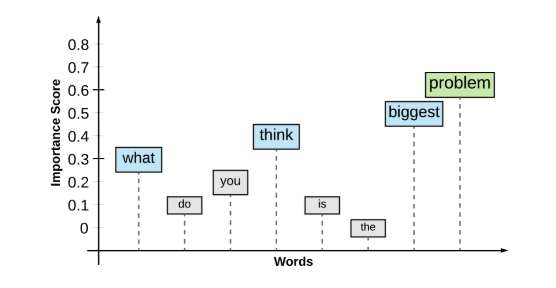
\includegraphics[width=15cm]{figures/word.png}
	\caption{An example of RIT annotation from S. Kafle and M. Huenerfauth, 2018}
	\label{fig:word}
\end{figure}

\section{Feature Extraction Tools} 
We use three software tools--Praat, ProsodyPro and Parselmouth to do prosodic feature extraction: Praat is a mainstream software tool for phonetic analysis; ProsodyPro is a Praat script that facilitates systemic analysis of speech prosody; Parselmouth is a Python interface to Praat which enables the whole procedure of this experiment, such as data processing and machine learning, be implemented in one programming language.

\subsection{ Praat}
Praat \citep{PaulBoersma&DavidWeenink2018} is a freeware program for the analysis and reconstruction of acoustic speech signals. The user is able to analyze, synthesize, manipulate speech and plot pictures for visualisation in papers. It was designed, and continues to be developed, by Paul Boersma and David Weenink of the University of Amsterdam. Praat is available for most platforms. The clear visual presentation of operational procedures and introduction to acoustic knowledge are provided to facilitate the users in linguistic research.

Some of its functionalities include:
\begin{itemize}
	\item generate waveforms, wide and narrow band spectrograms, intensity contour and pitch tracks;
	\item get information about pitch, intensity, formants, pulses and etc;
	\item enhance certain frequency regions; segment and label words, syllables, or individual phonemes;
\end{itemize}

\begin{figure}[ht]
	\center
	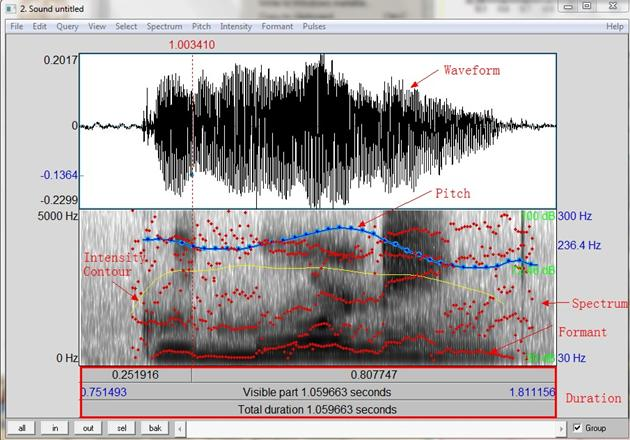
\includegraphics[width=10cm, scale=0.7]{figures/Praat.jpg}
	\caption{Speech analysis sofware Praat, from http://ec-concord.ied.edu.hk/}
	\label{fig:praat}
\end{figure}

http://www.fon.hum.uva.nl/praat/

\subsection{ProsodyPro}
ProsodyPro is a software for large-scale speech prosody analysis. The program is a Praat script developped by Yi Xu at University College London. It allows users to combine detailed analysis of continuous prosodic features with systematic comparison with discrete measurements . The key design of the tool is to implement time-normalisation for continous prosody and generate rich output files for graphical or statistical analysis(citep xu 2014).

Fig: ProsodyPro workflow

http://www.homepages.ucl.ac.uk/~uclyyix/ProsodyPro/

\subsection{Parselmouth}
Parselmouth is an open-source Python library developped by (citet Yannick ) that provides interface to core functionality of Praat in Python. It focus on applications in audio manipulation, file manipulation, statistical analysis, data visualisation and integration of automated acoustic analysis into experimental design.

fig(example codes)


\begin{figure}[ht]
	\center
	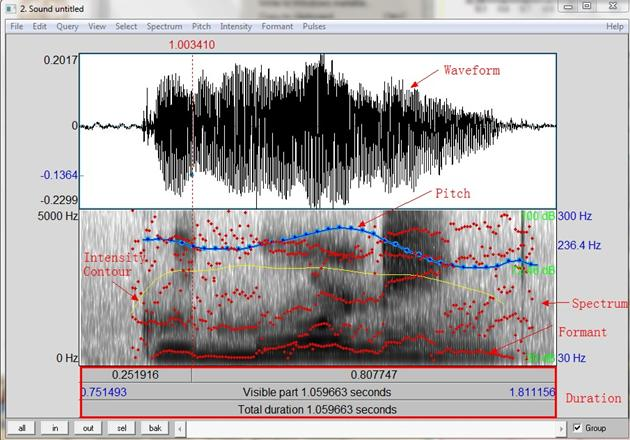
\includegraphics[width=10cm, scale=0.7]{figures/Praat.jpg}
	\caption{A code example of using Parselmouth to increase the fundamental frequency, from citet. Usage of Parselmouth functionality is highlighted in red}
	\label{fig:Parselmouth}
\end{figure}

Since Parselmouth is under developping, some classes such as PitchTier are not yet ready-to-use as ordinary Python objects, but the parselmouth.praat.call () function serves as an interface to Praat commands as it is shown in fig().

https://github.com/YannickJadoul/Parselmouth

\section{Feature Selection}
In this research, we extracted 11 word-level acoustic-prosodic features which are the default non-timenormalised feature setting of ProsodyPro. Features and their description are summarised in table()

table(feature list)

According to Section 2.1.3, we name excursion size, duration, mean intensity, max velocity, final velocity and max f0 location as more related features to prosodic prominence.

\section{Algorithms}
Spearman Rank Order Correlation Coefficient
pearson, spearman, kadel?
spearman is suitable
equation
numpy faster than pandas

stemming: nltk.stem.lancaster
http://www.nltk.org/_modules/nltk/stem/lancaster.html

stop words: nltk stop word list


tf-idf: sklearn.feature_extraction.text.TfidfVectorizer
https://scikit-learn.org/stable/modules/generated/sklearn.feature_extraction.text.TfidfVectorizer.html

Spearman Correlation: scipy.stats.spearmanr
https://docs.scipy.org/doc/scipy-0.14.0/reference/generated/scipy.stats.spearmanr.html




\section{Ethical, Professional and Legal Issues}
%\lipsum  % Replace with your text
This project will be implement according to the BSC Code of Conduct with a commitment to the author's professional integrity and in the public interest.

\begin{itemize}
	
	\item The data to use in this project is from public database, e.g. Switchboard corpus, and the software to use is open-source, e.g. Praat. The author will have due regard for public interest including privacy, equality and  the legitimate rights of Third Parties.
	
	\item This project will be done within the author's professional competence without stealing, copying or reproducing the work of others.
	
	\item The author promise to carry out his professional responsibilities with due care and
	diligence in accordance with the Relevant Authority’s requirements and will not misrepresent any data or information.
	
	\item The author will commit to the duty of his profession and seek to improve professional standards.
\end{itemize}



